% 
% El proyecto ha logrado parametrizar 
% en una medida considerable la simulación de la 
% plataforma Gough Stewart, con lo que se vuelve fácil 
% evaluar una infinidad de variaciones del sistema.
% Esta parametrización ya ha demostrado sus ventajas 
% en la etapa de pruebas de la interfaz gráfica.
% La posibilidad de estudiar el comportamiento del
% sistema a diferentes escalas ha permitido 
% identifix car errores en el comportamiento del 
% simulador y corregir dichos errores de manera adecuada.
% 


\section{Resultados}

Las estrategias de control implementadas fueron probadas con dos casos de prueba: posición final y seguimiento de trayectoria.
El caso de posición final evaluó el tiempo de estabilización y el error en estado estable del sistema.
El caso de seguimiento de trayectorias evaluó qué tan robusto
es el sistema y el comportamiento del mismo fuera del punto de linearización.

\subsection{Control PD}

\begin{figure}
    \centering
    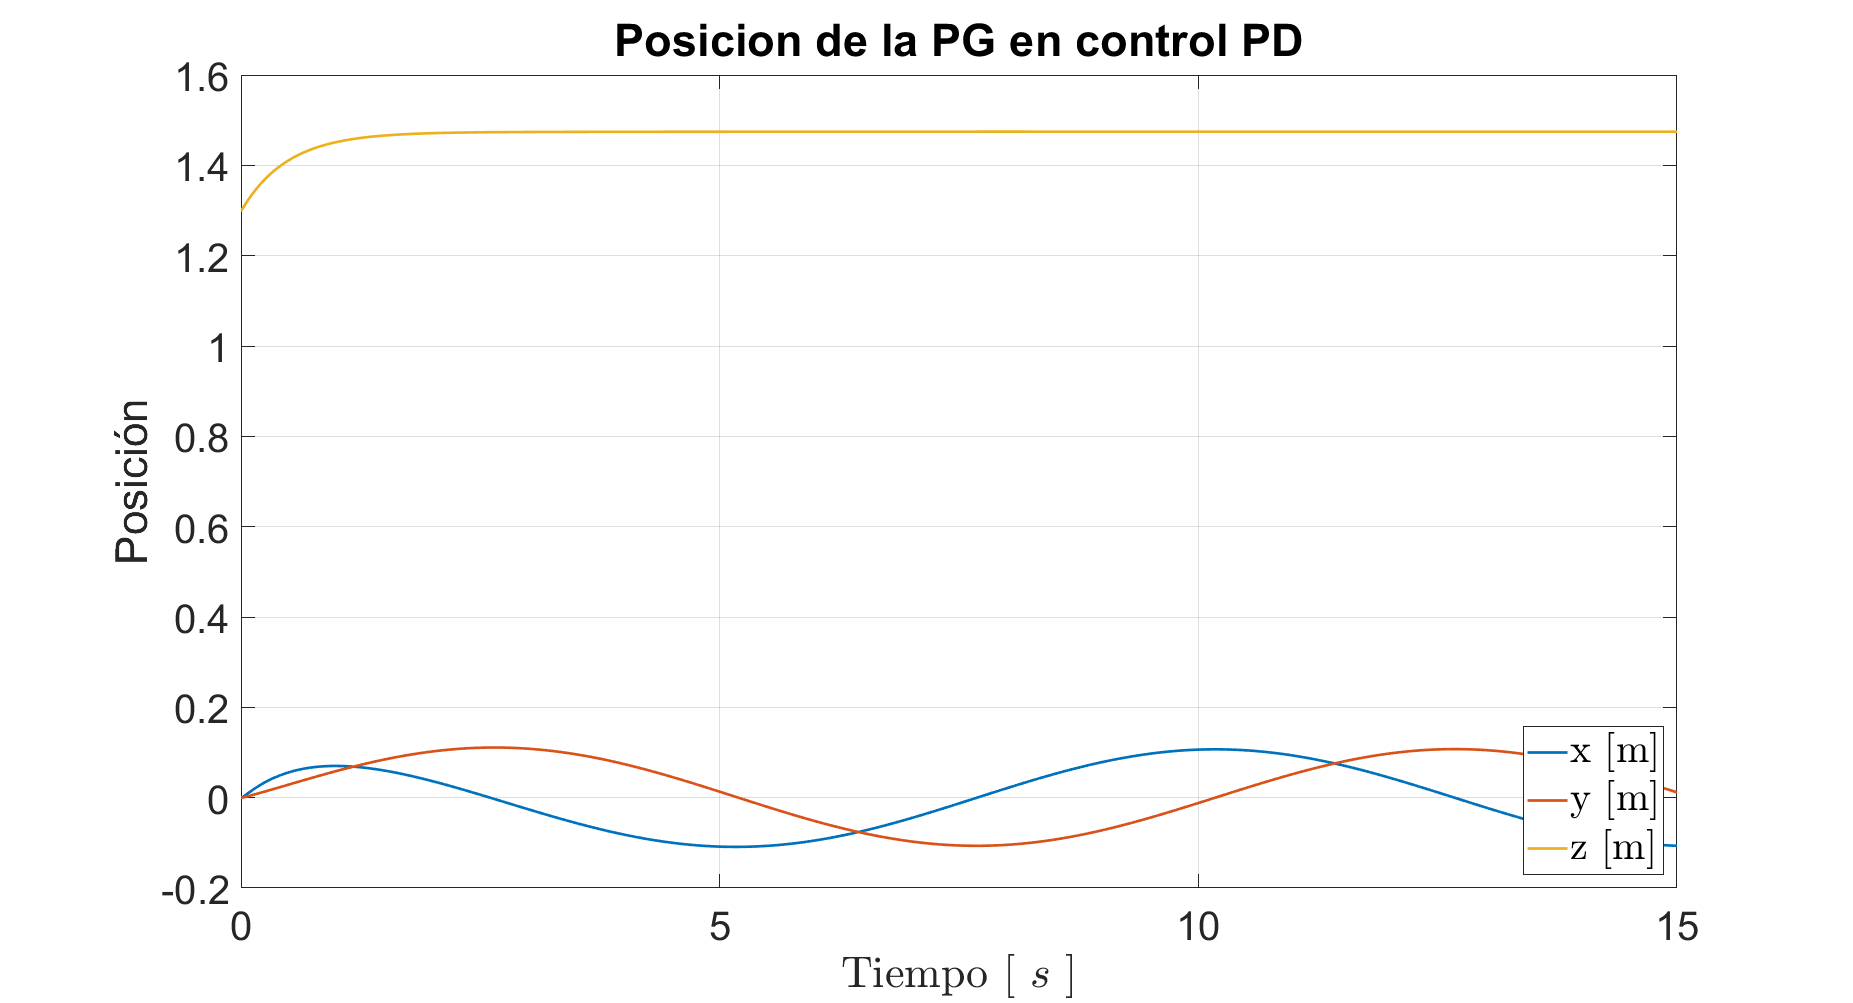
\includegraphics[width=0.4\textwidth]{posPD.png}
    \caption{Posición del sistema - PD.}
    \label{fig:PD position}
\end{figure}

\begin{figure}
    \centering
    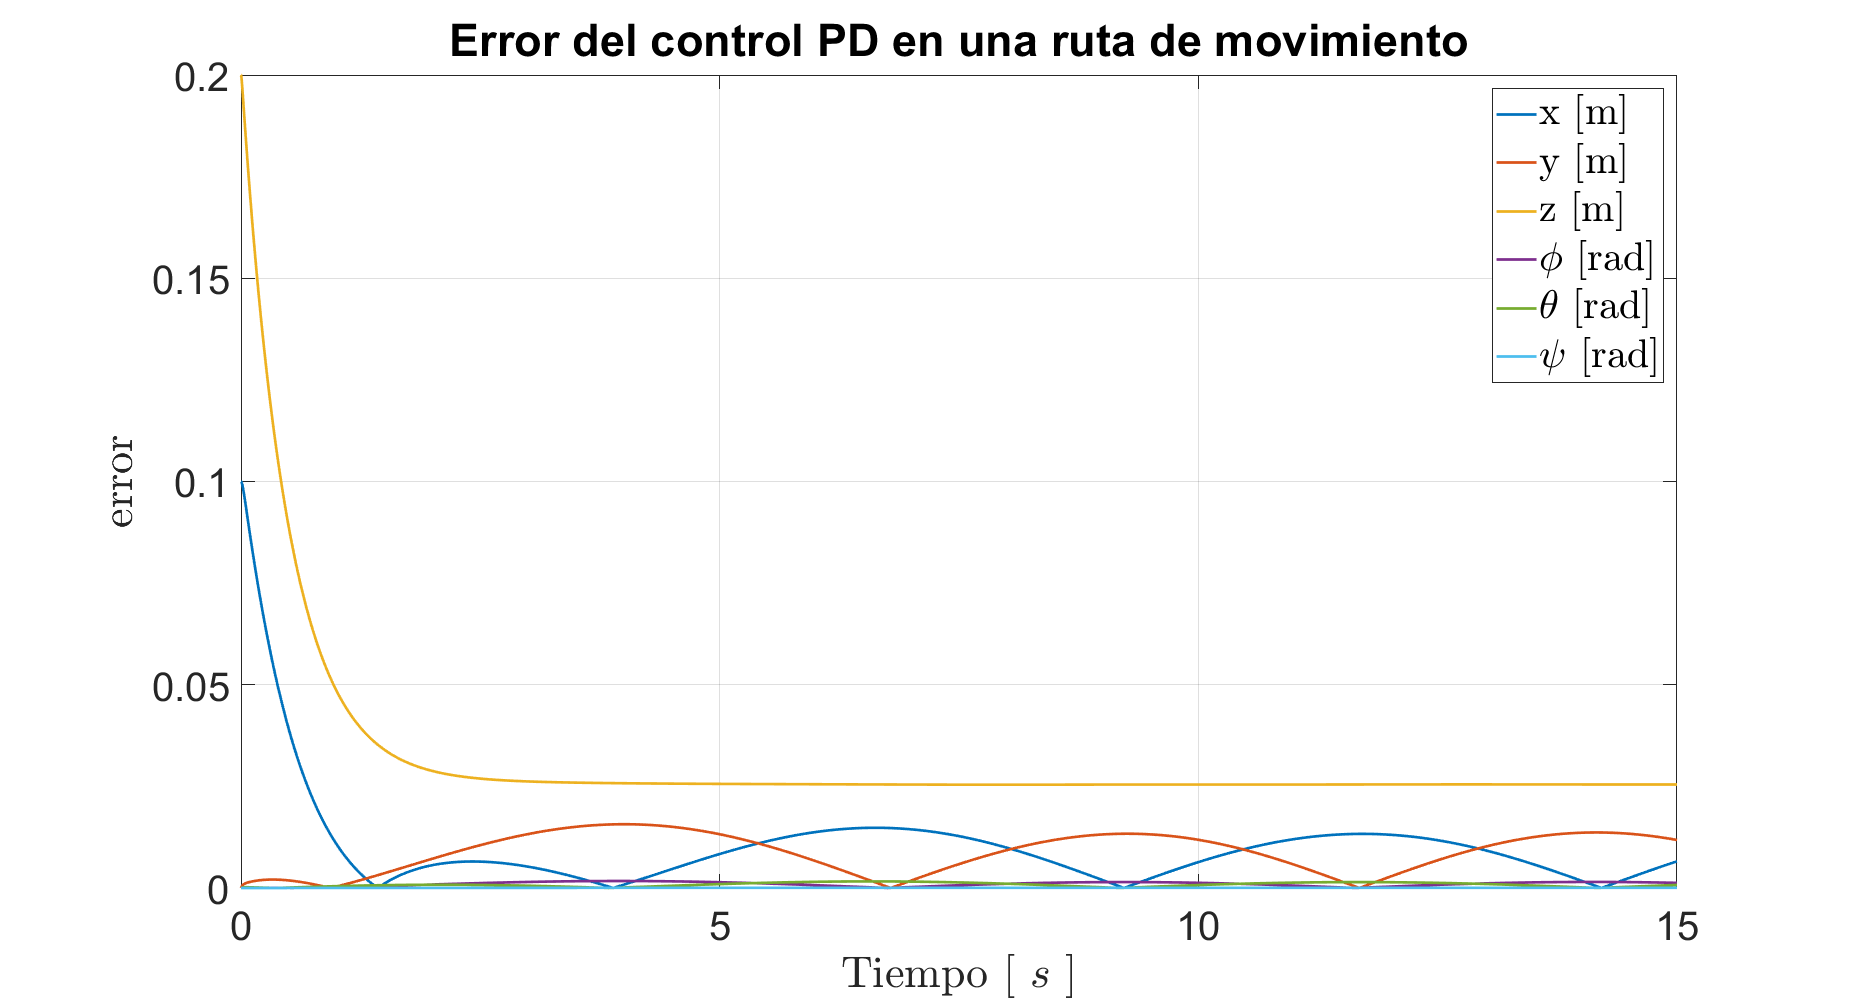
\includegraphics[width=0.4\textwidth]{errorPD.png}
    \caption{Error del sistema - PD.}
    \label{fig:PD error}
\end{figure}

\subsection{Control PD+G}

\begin{figure}
    \centering
    % 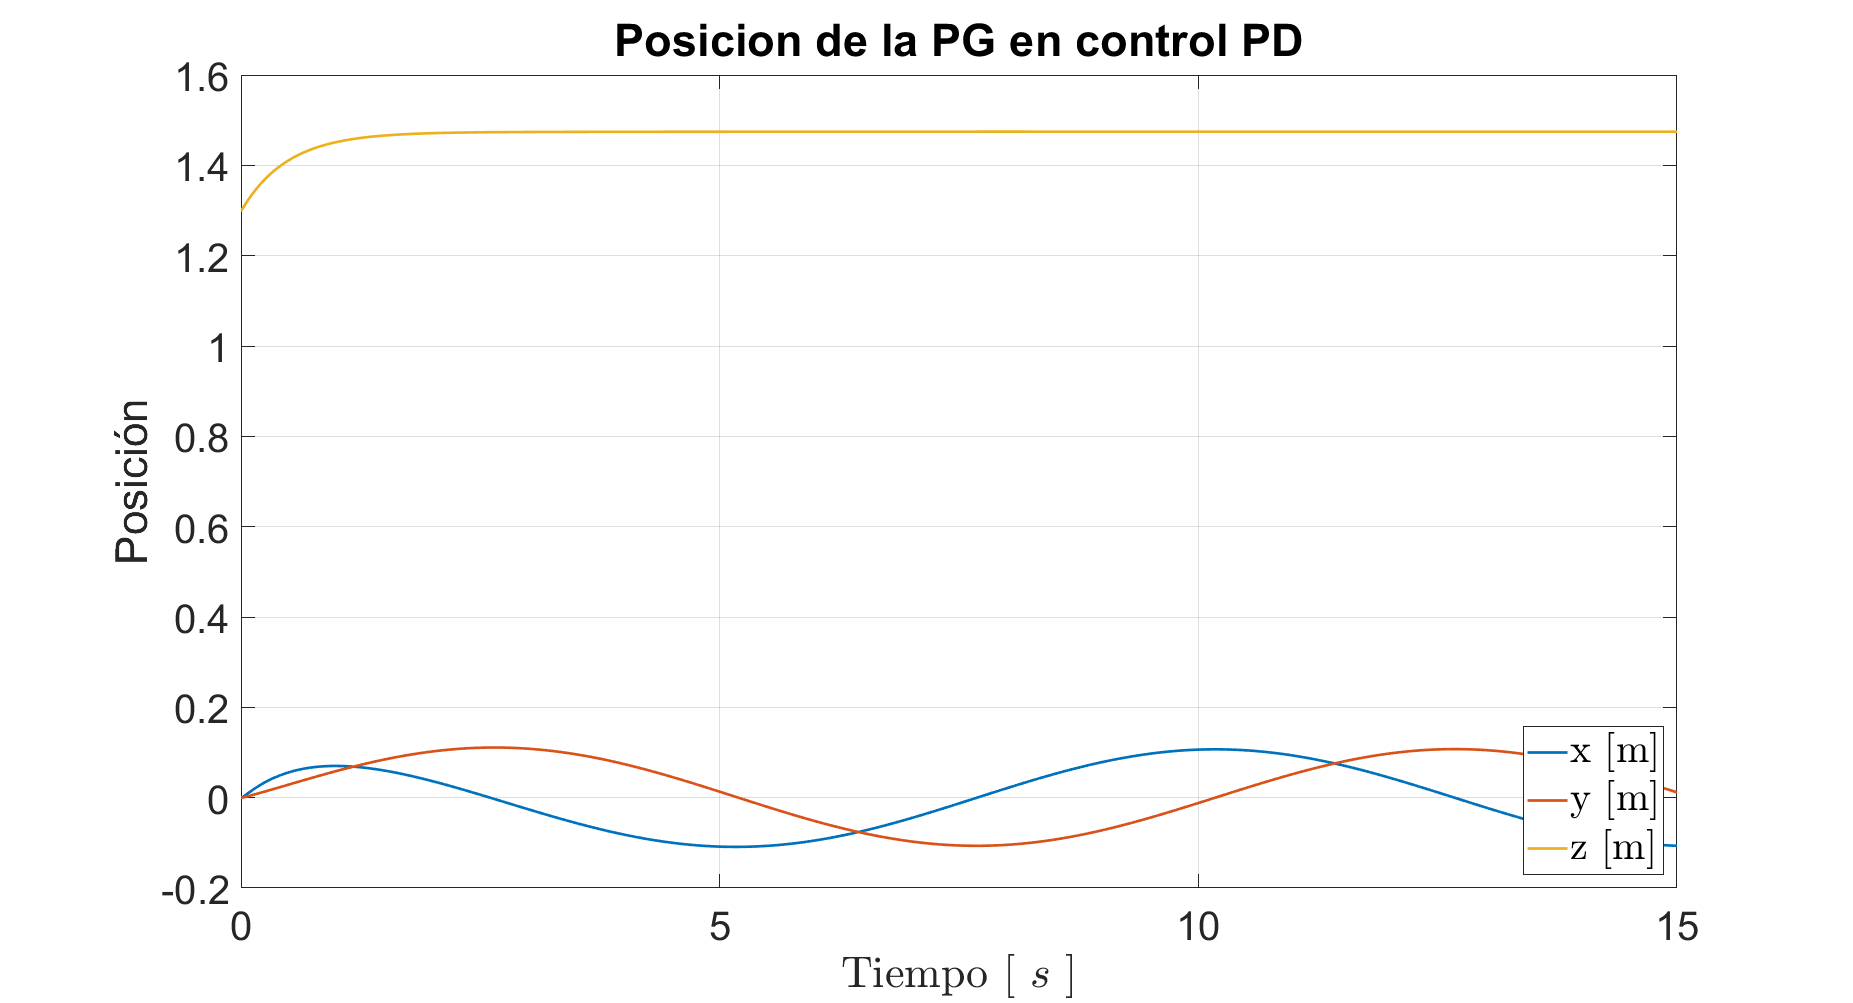
\includegraphics[width=0.4\textwidth]{posPD.png}
    \caption{Posición del sistema - PD+G.}
    \label{fig:PDG position}
\end{figure}

\begin{figure}
    \centering
    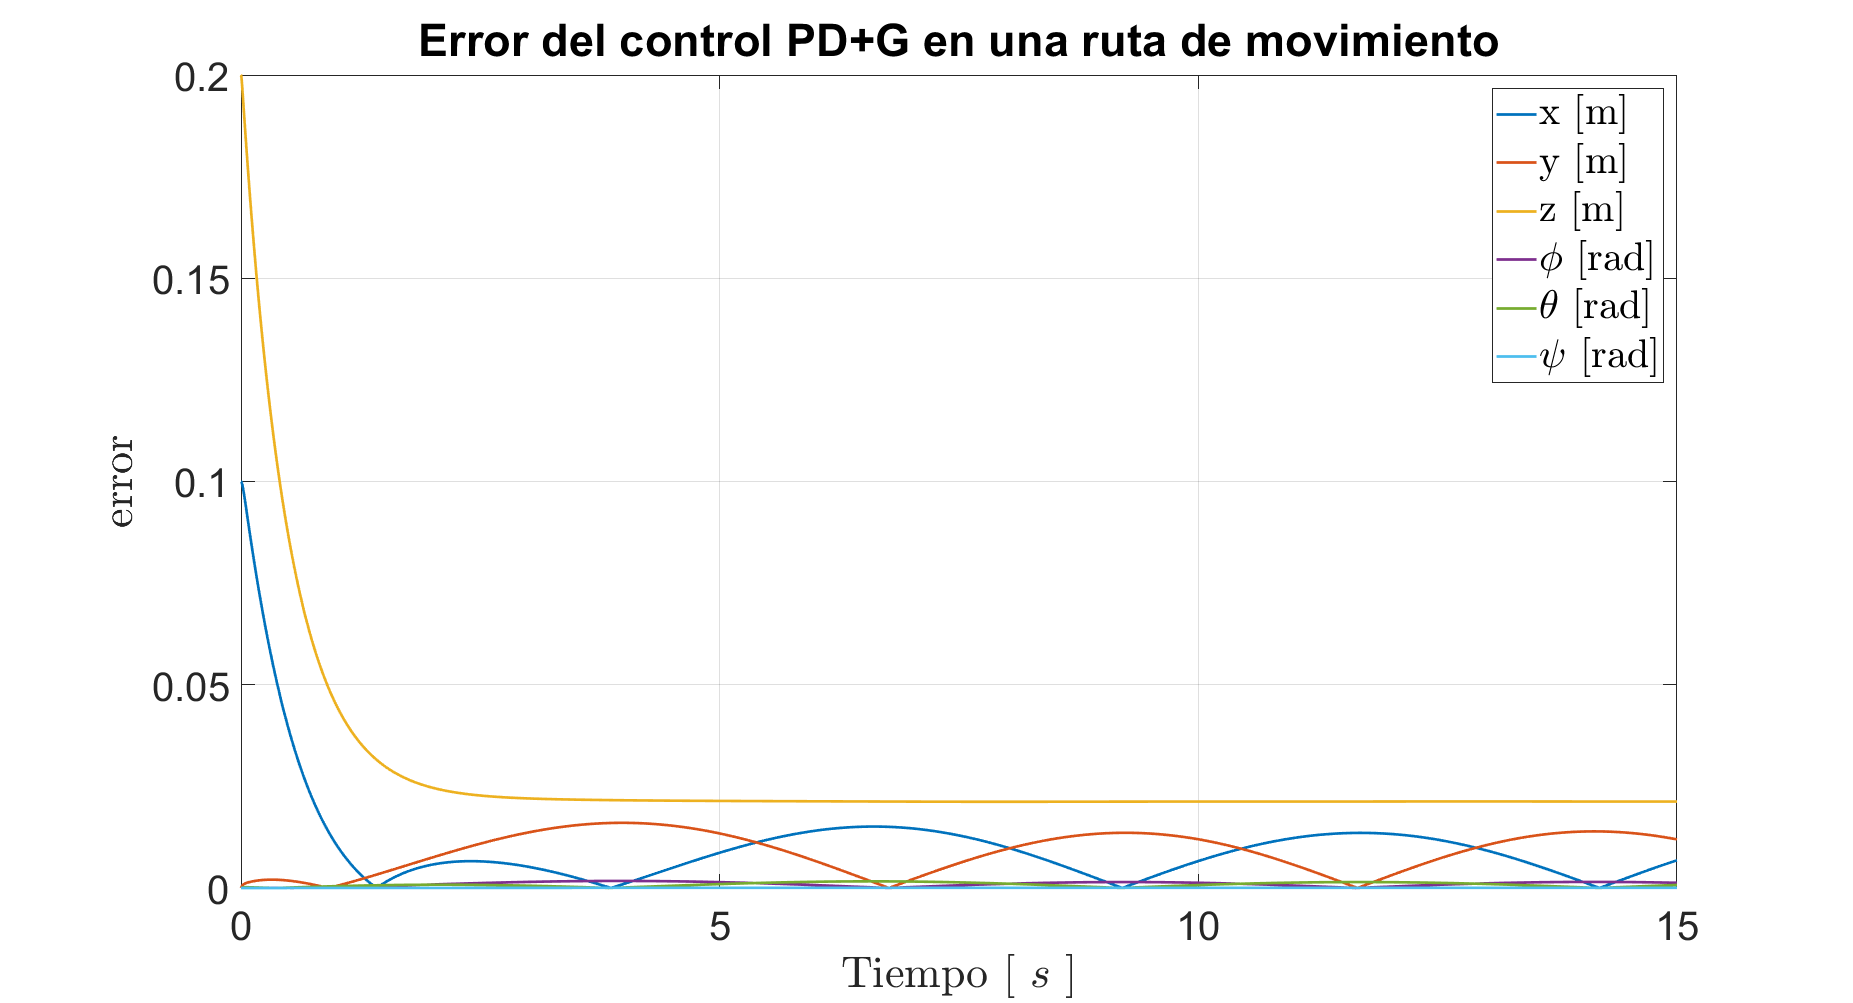
\includegraphics[width=0.4\textwidth]{errorPDpG.png}
    \caption{Error del sistema - PD+G.}
    \label{fig:PDG error}
\end{figure}


\subsection{Control PID}

\begin{figure}
    \centering
    % \includegraphics{}
    \caption{Posición del sistema - PID.}
    \label{fig:PID position}
\end{figure}

\begin{figure}
    \centering
    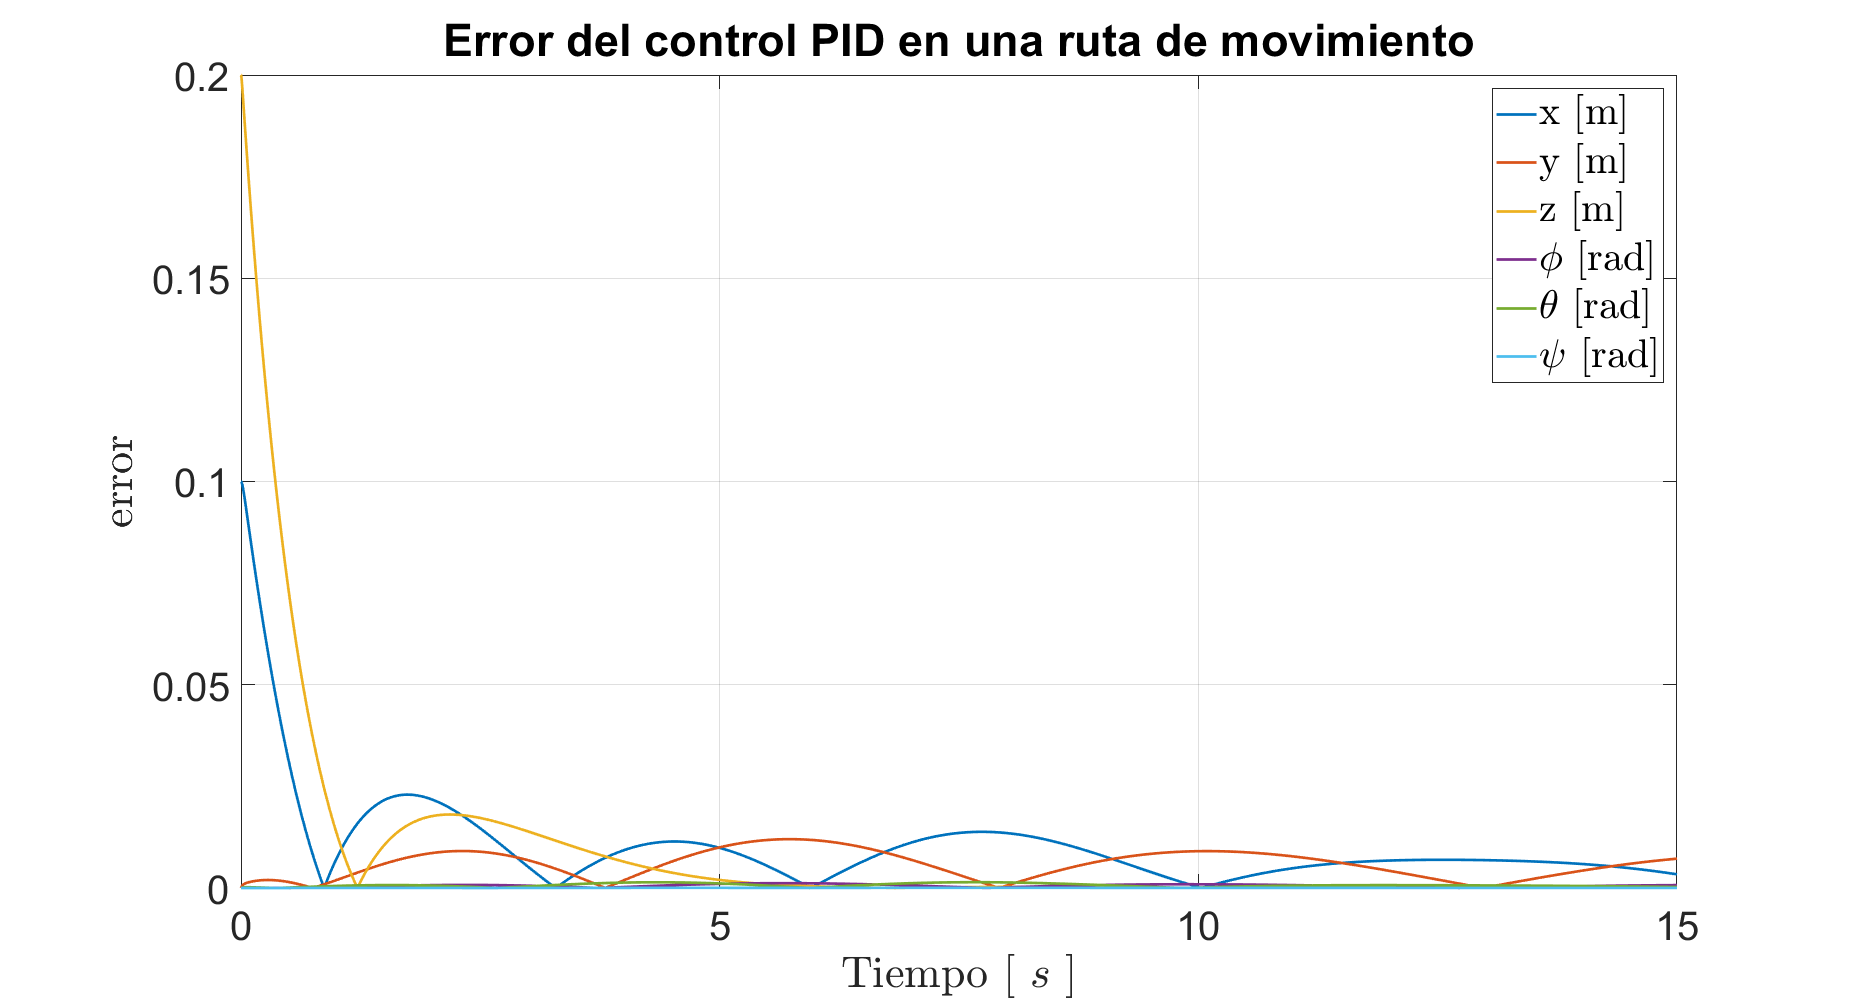
\includegraphics[width=0.4\textwidth]{errorPID.png}
    \caption{Error del sistema - PID.}
    \label{fig:PID error}
\end{figure}
